\subsection{Rotation Effect}
\label{sect:rotate}

In this task, you will create a rotation effect on an image.  The
core of this transformation is this function:
\begin{quote}
\begin{lstlisting}
pixel_t[] rotate(pixel_t[] pixels, int width, int height)
\end{lstlisting}
\end{quote}
The returned array should be the array representation of the
duplicated and rotated image.  An example of this transformation is given in
Figure~\ref{fig:carnegie-rotate}.

Your task here is to implement a function that takes as input an image
of size $w \times h$ and creates a ``rotation'' image of size $(w+h)
\times (w+h)$ that contains the same image repeated four times, the top
right image containing the original image, the top left containing the
original image rotated 90 degrees counterclockwise, the bottom left
containing the original image rotated 180 degrees, and the bottom
right containing the original image rotated 90 degrees clockwise.

The original image must have the same width and height in order to do the
``rotation'' effect, i.e., $w=h$. If the supplied image is not ``square''
(i.e., its width does not equal its height) or does not match the size given
by the given width and height, your function should abort with a precondition
failure when compiled and run with the \lstinline'-d' flag.

\begin{figure}
\centering
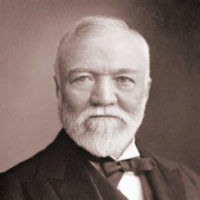
\includegraphics[scale=0.475]{\img/carnegie.png}
%\\[8em]
\quad\quad
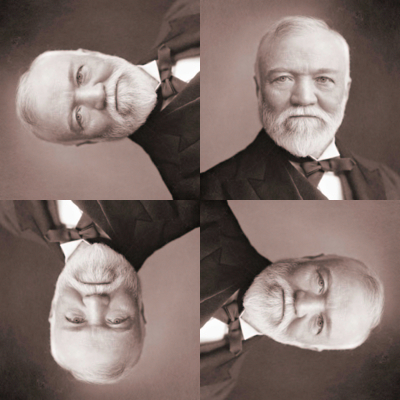
\includegraphics[scale=0.5]{\img/carnegie-rotate.png}
\caption{Original image (left); Image after ``rotation effect''}
\label{fig:carnegie-rotate}
\end{figure}

\begin{task}[8]
\TAGS{array, correctness, safety, testing}
  Create a C0 file \lstinline'rotate.c0' implementing a function
  \lstinline'rotate'.  You may include any auxiliary functions you
  need in the same file, but you should not include a
  \lstinline'main()' function.
\end{task}

You should look at \lstinline'README.txt' to see how to compile and run
this transformation against \lstinline'rotate-main.c0'.  You are also
strongly encouraged to write some test cases for your
programs in \lstinline'images-test.c0'.




%%% Local Variables:
%%% mode: latex
%%% TeX-master: "main"
%%% End:
